W pracy założono, że pojazdy rolnicze w przybliżeniu są bryłami sztywnymi.
Obiekty te charakteryzują się w przestrzeni trójwymiarowej sześcioma stopniami swobody.
Jednym ze sposobów matematycznego opisu położenia tychże pojazdów w przestrzeni trójwymiarowej,
jest podanie współrzędnych środka ciężkości (x,y,z) oraz trzech parametrów kątowych: azymutu, odchylenia od poziomu w płaszczyźnie poprzecznej oraz podłużnej.
W dalszej części rozdziału opisano kilka przykładowych rozwiązań algorytmów sterowania,które charakterytzują się różnym podejściem 
w odniesieniu do parametrów kątowych określania orientacji przestrzennej pojazdów rolniczych. 
\section{Podział algorytmów sterowania ze względu na dostarczane dane wejściowe}
Jednym z najbardziej popularnych zbiorów parametrów nawigacyjnych, które są następnie wysyłane do algorytmów sterowania, jest para:
azymut plus offset obliczane względem zadanej trasy. Azymut jest to kąt którego ramionami są:
główna oś symetrii pojazdu oraz styczna do krzywej prowadzenia w punkcie, który stanowi rzut prostopadły środka ciężkości na tą krzywą.
Offset natomiast jest to odległość środka ciężkości pojazdu względem zadanej ścieżki \cite{CCTA_769_775}.
Na rysunku nr \ref{fig:ch3_azymutOffset} przedstawione są powyższe parametry. Środek ciężkości pojazdu oznaczono jako C,
azymut pojazdu względem zadanej źcieżki oznaczono jako $\psi$. $\delta$ oznacza kąt sterujący jako wynik przetwarzania algorytmu sterującego tzw. Target Angle.    
\begin{figure}[H] 
\centering
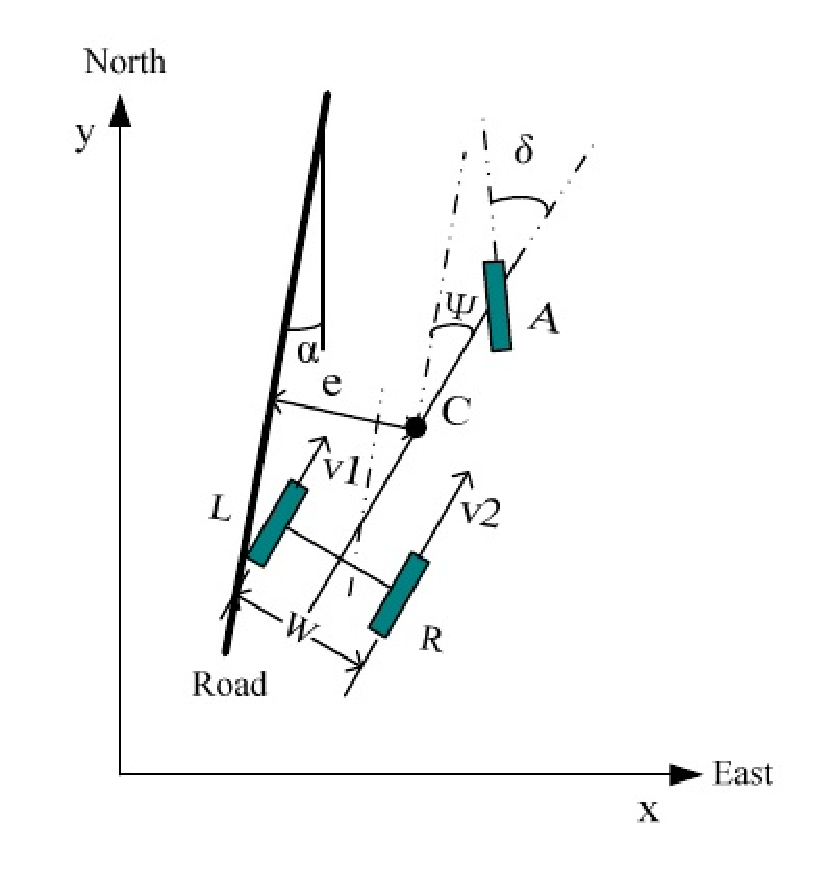
\includegraphics[scale=0.5]{ch3_azymutOffset.eps}
\caption{\textit{Azymut oraz offset - Parametry najczęściej używane w celu wyznaczenia pozycji względem zadanej trasy;}
źródło: \cite[][strona 464]{CCTA5_461_469}}
\label{fig:ch3_azymutOffset}
\end{figure}

W przypadku niskiej dokładności parametrów nawigacyjnych autorzy publikacji \cite{CCTA_943_950}
zaproponowali algorytm, który korzysta tylko z obliczanego w czasie rzeczywistym offsetu.
\begin{figure}[H]
\centering
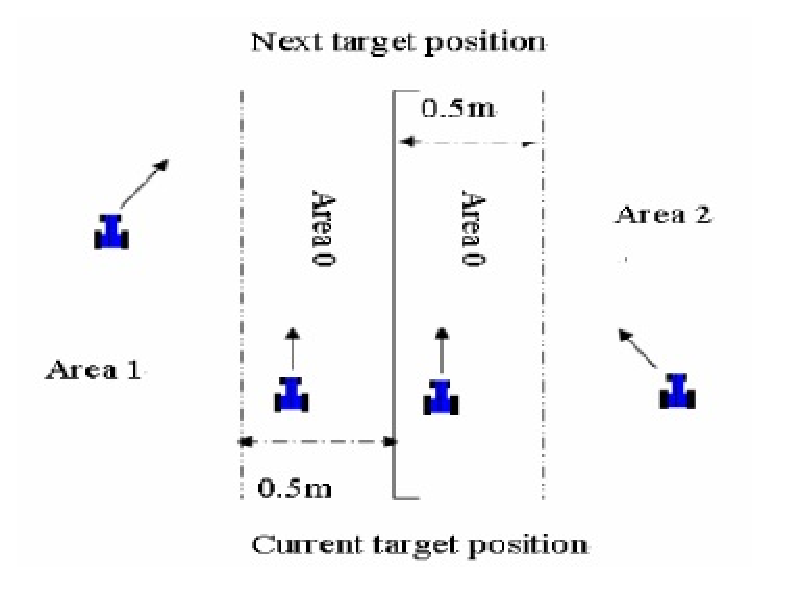
\includegraphics[scale=0.8]{ch3_currentNextTargetPosition.eps}
\caption{\textit{Tylko offset - w przypadku niskiej jakości danych wejściowych;} 
	źródło: \cite[][strona 947]{CCTA_943_950}}
\label{fig:ch3_currentNextTargetPosition}
\end{figure}

\indent W przypadku trudnych warunków pogodowych bądź obecności innych czynników powodujących poślizg kół pojazdu wymagana 
jest estymacja współczynników korygujących wyniki algorytmu sterującego \cite[]{KRAUS}. Poniższy rysunek \ref{fig:side_forward_slip} ilustruje modelowanie 
poślizgu w płaszczyznach: poprzecznej oraz podłużnej.

\begin{figure}[H]
\centering
\begin{subfigure}{.4\textwidth}
  \centering
  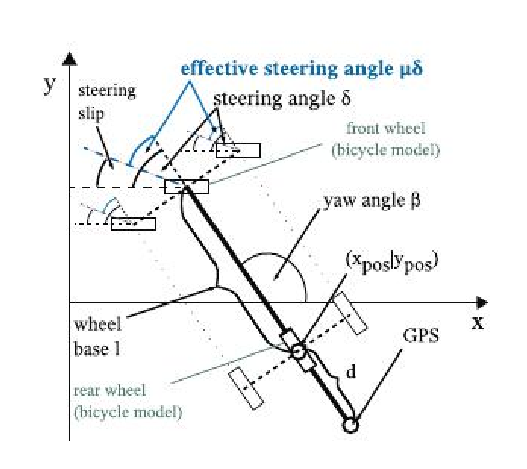
\includegraphics[width= 1.2\linewidth]{ch3_effective_stearing_angle.eps}
  \caption{Schemat przedstawiający zaadaptowanie modelu pojazdu jednosiowego z poślizgiem bocznym (w postaci zmiany kąta sterującego), do opisu ciągnika rolniczego}
  \label{fig:side_slip}
\end{subfigure}
\hspace{2cm}
\begin{subfigure}{.4\textwidth}
  \centering
  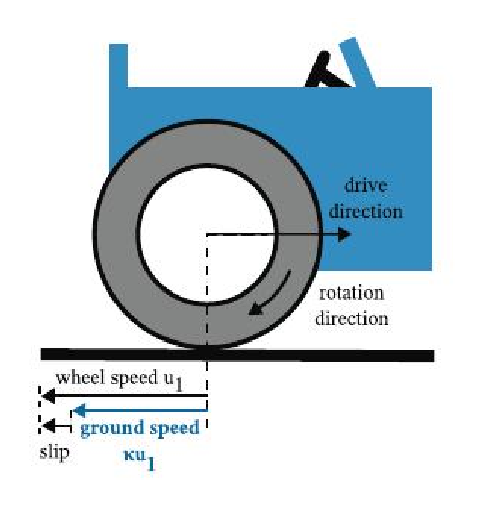
\includegraphics[width= 1.2\linewidth]{ch3_effective_wheel_speed.eps}
  \caption{Modelowanie poślizgu ciągnika w płaszczyźnie podłużnej}
  \label{fig:longitudinal_slip}
\end{subfigure}
\caption{\textit{Estymacja parametrów $\kappa$ oraz $\mu$ pozwalających na poprawne prowadzenie pojazdu w warunkach obecności poślizgu.}
źródło powyższych rysunków: \cite[][strona 26]{KRAUS}}
\label{fig:side_forward_slip}
\end{figure}

\section{Podział algorytmów sterowania ze względu na zastosowane algorytmy decyzyjne}
Różnego rodzaju algorytmy sterowania są używane w celu kompencacji zmiennej dynamiki pojazdów oraz w celu osiągnięcia satysfakcjonującej wydajności sterowania
 \cite[][strona 770]{CCTA_769_775}. Poniżej znajdują się przykłady kilku najbardziej popularnych algorytmów prowadzenia pojazdów.

\begin{wrapfigure}[15]{o}[20pt]{8cm}
	\centering
	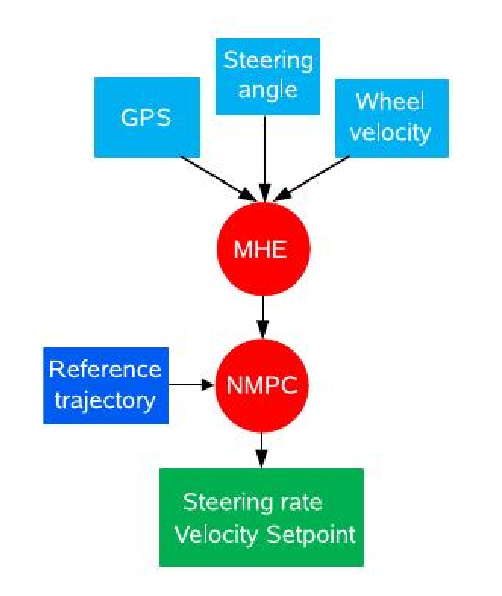
\includegraphics[scale = 0.9]{ch3_MHE_NMPC_estimation.eps}
	\caption{\textit{Schemat blokowy zaawansowanego algorytmu prowadzenia pojazdu dostosowanego do występowania poślizgu kół.}
	źródło \cite[][strona 30]{KRAUS}}
	\label{fig:MHE_NMPC_diagram}
\end{wrapfigure}
\indent W pracy \cite[]{KRAUS} Tom Kraus wraz z współpracownikami opisali zaawansowany matematycznie algorytm wyznaczania parametrów prowadzenia 
ciągnika rolniczego - zmiany kąta sterowania oraz prędkości kątowej kół pojazdu, przy użyciu estymacji z przesówanym oknem czasowym (MHE\footnote{
Moving Horizon Estimation}) oraz nieliniowym modelem predykcyjnego sterowania (NMPC\footnote{Nonlinear Model Predictive Control}).
Wektor stanu poruszającego się obiektu, zawierający niewiadome $\kappa$, $\mu$ opisujące poślizg \ref{fig:side_forward_slip}, oraz orientację,
estymowany był za pomocą algorytmu MHE. Na podstawie znajomości aktualnego stanu obiektu oraz trasy referencyjnej algorytm predykcyjny NMPC wyznaczał wynikowe parametry 
prowadzenia pojazdu \cite[][strona 30]{KRAUS}. Rysunek \ref{fig:MHE_NMPC_diagram} przedstawia schemat blokowy opisanego algorytmu. 
Sterowanie predykcyjne z przesówanym oknem czasowym, polega na cyklicznym rozwiązywaniu zadania sterowania optymalnego, z warunkiem początkowym 
równym aktualnej estymacie stanu obiektu \cite[][strona 2]{BANIA}. Predykcja przyszłych stanów obiektu sterowanego na podstawie nieliniowych równań różniczkowych jest możliwa 
tylko w stosunkowo krótkim oknie czasowym przyjmowanym arbitralnie - stąd nazwa metody.

